\section{Theorie 502}

\subsection{Berechnung der Elektronenbahn im homogenen Magnetfeld}
Anders als im elektrischen Feld wirkt auf ein Elektron im Magnetfeld nur eine Kraft, wenn sich das Elektron durch dieses bewegt. Diese Kraft wird Lorentzkraft genannt. Bewegt sich eine Ladung $q$ durch ein homogenes Magnetfeld 
$\vec{B}$ mit der Geschwindigkeit $\vec{v}$, dann lässt sich die Lorentzkraft mit

\begin{equation}
\vec{F_{\text{L}}} = q \vec{v} \times \vec{B}
\label{eqn:lorentz}
\end{equation}
berechnen. 

Gegeben ist ein Magnetfeld, dessen Feldlinien parallel zur X-Achse eines kartesischen Koordinatensystems ausgerichtet sind. Bewegt sich nun ein Elektron mit der Ladung $e_0$ und der Masse $m_0$ mit der Geschwindigkeit $\vec{v_0}$ 
in Z-Richtung durch das Magnetfeld, so wirkt auf ihn die Lorentzkraft in Y-Richtung:

\begin{equation} 
F_{\text{L}_{\text{y}}} = e_0 v_0 B.
\end{equation}

Da laut \ref{eqn:lorentz} die Kraft stets senkrecht zum Wegelement $\symup{d}\vec{s}$ steht, ist

\begin{equation}
\vec{F_{\text{L}}} \cdot \symup{d}\vec{s} = 0
\end{equation}
und damit bleibt die potentielle Energie und daraus folgernd auch die kinetische Energie des Elektrons konstant. Zudem ist wegen

\begin{equation}
E_{\text{kin}} = \frac{1}{2} m_0 v^2
\end{equation}
$\abs{\vec{v}}$ ebenfalls immer konstant und in allen Bahnpunkten gilt

\begin{equation}
\abs{\vec{v}} = v_0.
\end{equation}

In einem Magnetfeld ist die auf das Elektron wirkende Kraft gleich der Zentripetalkraft:

\begin{equation}
e_0 v_0 B = \frac{m_0 \abs{\vec{v}}^2}{r}.
\end{equation}
Wird die Gleichung nach dem Radius $r$ umgestellt, dann zeigt sich, dass sich aufgrund eines konstanten Radius das Elektron auf einer Kreisbahn bewegt:

\begin{equation}
r = \frac{m_0 v_0}{e_0 B}
\label{eqn:radius}
\end{equation}




\subsection{Experimentelle Bestimmung der spezifischen Elektronenladung}

Die spezifische Ladung $\frac{e_0}{m_0}$ kann mit der Kathodenstrahlröhre bestimmt werden. Dazu werden die Elektronen mit der Beschleunigungsspannung $U_{\text{B}}$ auf eine Geschwindigkeit $v_0$ gebracht:

\begin{equation}
v_0 = \sqrt{2U_{\text{B}} \frac{e_0}{m_0}}.
\label{eqn:geschwindigkeitspannung}
\end{equation}

\begin{figure}[h!]
	\centering
	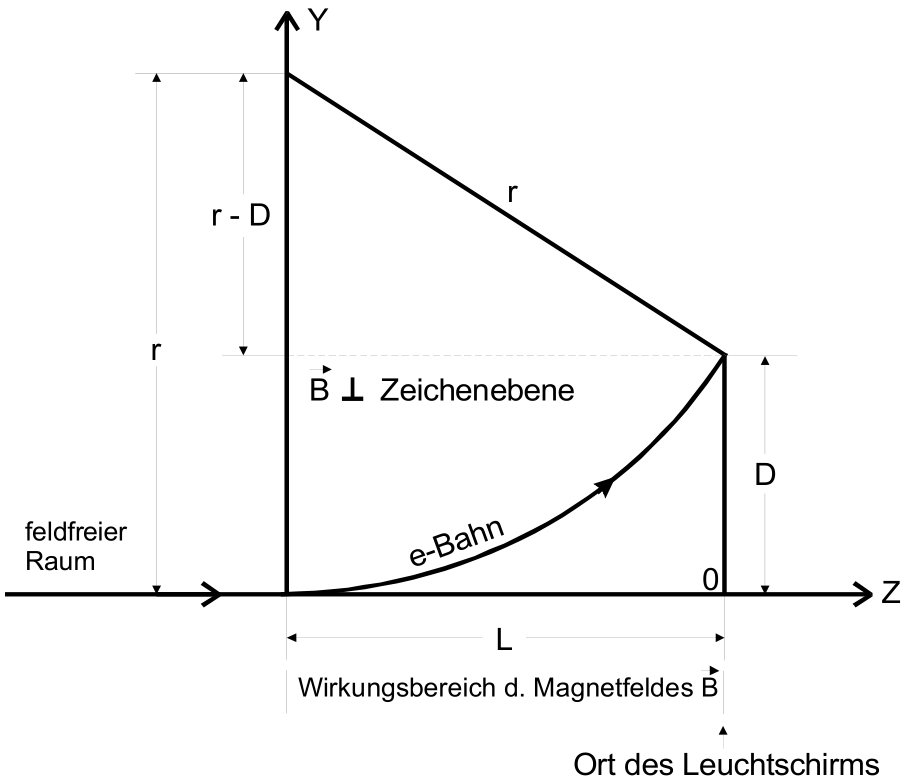
\includegraphics[width=0.8\linewidth]{bahnkurve.png}
	\caption{Skizze zur Ableitung einer Beziehung zwischen L, D und r.}
	\label{fig:bahnkurve}
\end{figure}

Im Magnetfeld bewegen sich die Elektronen aufgrund der Lorentzkraft auf einer gekrümmten Bahn und treffen dann auf den Leuchtschirm der Kathodenstrahlröhre. Die Verschiebung vom Mittelpunkt des Schirms, also dem Punkt, den der Strahl
in einem feldfreien Raum träfe, wird nun als $D$ bezeichnet. Die Verschiebung kann mithilfe des Satzes des Pythagoras aus dem Radius $r$ der Kreisbahn und der Länge $L$ des Wirkungsbereichs des Magnetfeldes errechnet werden:

\begin{equation}
\begin{aligned}
r^2 &= L^2 + (r-D)^2 \\
\iff r &= \frac{L^2 + D^2}{2D}
\label{eqn:radiuspythagoras}
\end{aligned}
\end{equation}
Nun kann \ref{eqn:radiuspythagoras} in \ref{eqn:radius} eingesetzt werden, woraus sich

\begin{equation}
\frac{m_0 v_0}{e_0 B} = \frac{L^2 + D^2}{2D} 
\end{equation}
ergibt. Außerdem lässt sich auch die Geschwindigkeit $v_0$ mithilfe von \ref{eqn:geschwindigkeitspannung} ersetzen:

\begin{equation}
\frac{m_0}{e_0 B} \sqrt{2 U_{\text{B}} \frac{e_0}{m_0}} = \frac{L^2 + D^2}{2D}
\end{equation}
beziehungsweise

\begin{equation}
\frac{D}{L^2 + D^2} = \frac{1}{\sqrt{8 U_{\text{B}}}} \sqrt{\frac{e_0}{m_0}} B.
\end{equation}
